% !TEX spellcheck = en_US
% !TEX spellcheck = LaTeX
\documentclass[a4paper,10pt,english]{article}
\usepackage{%
	amsfonts,%
	amsmath,%	
	etex,%
	amssymb,%
	amsthm,%
	babel,%
	bbm,%
	%biblatex,%
	caption,%
	centernot,%
	color,%
	enumerate,%
	epsfig,%
	epstopdf,%
	geometry,%
	graphicx,%
	hyperref,%
	latexsym,%
	mathtools,%
	multicol,%
	pgf,%
	pgfplots,%
	pgfplotstable,%
	pgfpages,%
	proof,%
	psfrag,%
	subfigure,%	
	tikz,%
	ulem,%
	url%
}	

\usepackage[mathscr]{eucal}
\usepgflibrary{shapes}
\usetikzlibrary{%
  arrows,%
	backgrounds,%
	chains,%
	decorations.pathmorphing,% /pgf/decoration/random steps | erste Graphik
	decorations.text,%
	matrix,%
  	positioning,% wg. " of "
  	fit,%
	patterns,%
  	petri,%
	plotmarks,%
  	scopes,%
	shadows,%
  	shapes.misc,% wg. rounded rectangle
  	shapes.arrows,%
	shapes.callouts,%
  	shapes%
}

\theoremstyle{plain}
\newtheorem{thm}{Theorem}[section]
\newtheorem{lem}[thm]{Lemma}
\newtheorem{prop}[thm]{Proposition}
\newtheorem{cor}[thm]{Corollary}

\theoremstyle{definition}
\newtheorem{defn}[thm]{Definition}
\newtheorem{conj}[thm]{Conjecture}
\newtheorem{exmp}[thm]{Example}
\newtheorem{assum}[thm]{Assumptions}
\newtheorem{axiom}[thm]{Axiom}

\theoremstyle{remark}
\newtheorem{rem}{Remark}
\newtheorem{note}{Note}

\newcommand{\norm}[1]{\left\lVert#1\right\rVert}
\newcommand{\indep}{\!\perp\!\!\!\perp}
\DeclarePairedDelimiter\abs{\lvert}{\rvert}%
%\DeclarePairedDelimiter\norm{\lVert}{\rVert}%
\newcommand{\tr}{\operatorname{tr}}
\newcommand{\R}{\mathbb{R}}
\newcommand{\Q}{\mathbb{Q}}
\newcommand{\N}{\mathbb{N}}
\newcommand{\E}{\mathbb{E}}
\newcommand{\Z}{\mathbb{Z}}
\newcommand{\B}{\mathscr{B}}
\newcommand{\C}{\mathcal{C}}
\newcommand{\T}{\mathscr{T}}
\newcommand{\F}{\mathcal{F}}
\newcommand{\G}{\mathcal{G}}
%\newcommand{\ba}{\begin{align*}}
%\newcommand{\ea}{\end{align*}}

\makeatletter
\def\th@plain{%
  \thm@notefont{}% same as heading font
  \itshape % body font
}
\def\th@definition{%
  \thm@notefont{}% same as heading font
  \normalfont % body font
}
\makeatother
\date{}
\usepackage{placeins}
\newcommand\Mycomb[2][n]{\prescript{#1\mkern-0.5mu}{}C_{#2}}
\begin{document}
\begin{titlepage}
	\centering
	
\includegraphics[width=0.2\textwidth]{images.png}\par\vspace{1cm}
	{\scshape\LARGE Indian Institute of Science \par}
	\vspace{1cm}
	{\scshape\Large Submitted in partial fulfilment of the course \\ E2 204- Stochastic Process and Queuing Theory\par}
	\vspace{1.5cm}
	{\huge\bfseries Mobile Ad-hoc networks\par}
	\vspace{2cm}
	{\Large\itshape Roshan Antony\par}
		{\Large\itshape Sireesha Madabhushi\par}
			{\Large\itshape Vinay Kumar B R\par}
	\vfill
	
	% Bottom of the page
	{\large \today\par}
\end{titlepage}
\tableofcontents
\section{Introduction}
\par Mobile communication today has evolved to handle high data rates and the need of the hour is to have reliable seamless communication. MANETs have become popular at this juncture and are ubiquitous due to the presence of mobiles and laptops. However a persistent problem in MANETs is to maintain connectivity given that the nodes are moving at high speeds. Such scenarios also arise in sensor networks and tactical networks such as UAVs, ships etc. wherein connectivity could be a single point of failure for the whole system.
\par In this project, we take a minor step in addressing these issues. We look into the networking properties of a bunch of nodes which are randomly moving on an integer lattice. We evaluate properties of this network such as the mean time for connectivity and the expected time for all the nodes to get certain information from a broadcasting node. In certain applications, the environment in which the nodes are present can be approximated to a lattice by restricting the communicating radius of the nodes.
\par An alternate application of these results could be in the process of secret sharing wherein a particular secret is divided among multiple parties(say $n$) and the whole secret could be recovered only if atleast a certain number(say $k$) of the individual parties come together. In this case the expected time for $k$-connectivity of the underlying graph is the same as the expected time for the secret to be leaked. 
\par In Section \ref{model}, we describe the network as well as the mobility model we are working with. In Section \ref{MC}, we describe the initial Markov chain approach to determine the expected time for connectivity. In Section \ref{bcast}, we give a characterization of the broadcast time in a finite lattice and analyze it when the source node is fixed or mobile. We show some simulations for multiple nodes in Section \ref{sim} and conclude with Sections \ref{concl} and \ref{fw}.

\section{System model}\label{model}
Our model consists of $m$ nodes distributed independently on an integer lattice from 0 to $L-1$. Each node executes a random walk. Let $X_i(n)$ denotes the location of node $i$ at time instant $n$. In the symmetric random walk, we have 
\begin{equation}
X_i(n+1)=
\begin{cases}
X_i(n)+1 &w.p. \frac{1}{2}\\
X_i(n)-1 &w.p. \frac{1}{2},
\end{cases}
\end{equation}
and in the asymmetric case 
\begin{equation}
X_i(n+1)=
\begin{cases}
X_i(n)+1 &w.p.\hspace{.5cm} p\\
X_i(n)-1 &w.p.\hspace{.5cm} 1-p.
\end{cases}
\end{equation}
Another class of mobility models that was explored was the lazy random walk where the probability of remaining in a particular spot is non-zero that is,
\begin{equation}
X_i(n+1)=
\begin{cases}
X_i(n)+1 &w.p.\hspace{.5cm} \frac{p}{2}\\
X_i(n)   &w.p.\hspace{.5cm} 1-p\\
X_i(n)-1 &w.p.\hspace{.5cm} \frac{p}{2}.
\end{cases}
\end{equation}
A node present at 0($L$-1) jumps to either 1($L$-2) or $L$-1(0) with probability $\frac{1}{2}$ in the symmetric case. Similarly in the asymmetric random walk, it jumps to the same states but with respective probabilities. In this report, we refer to this as the \textit{torus boundary conditions}.
\par It can easily be noted that with these boundary conditions, the motion of the nodes in 0 to $L$-1 can be viewed as the nodes executing the random walks on a circle with $L$ vertices from 0 to $L$-1. This is shown in figure \ref{circ}. Random walks on a circle have been studied widely(see \cite{circle2},\cite{diaconis}). However they do not address the case when there are multiple nodes on the circle. Typically questions like the last node to be visited once every vertex is covered are answered.
\par Two nodes moving on the circle are said to be connected when they are co-located at a lattice point at a particular time. We assume that when two nodes get connected each node gets the information that the other has before the next time instant.

\begin{figure}\label{circ}
	\centering
	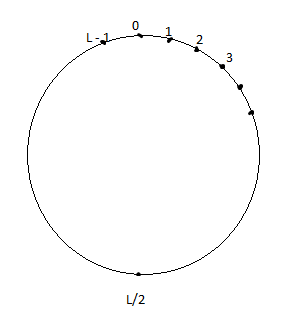
\includegraphics[scale = 0.5]{circle.png}
	\caption{Random walk on a finite lattice can be seen as random walk on a circle}
	\label{circ}
\end{figure}


\section{Connectivity- Markov chain approach}\label{MC}
The Markov chain for locations of various nodes needs to be positive recurrent to guarantee connectivity of the nodes. We now proceed with this line of thought to arrive at an expression for probability of the Markov chain recurring to the connected state \cite{ross}.\\
On a circle, we have irreducible and finite state space but not periodicity.
But if there are odd number of points on the circle, then the underlying Markov chain is aperiodic and hence positive recurrent.
If the circle has even number of points, positive recurrence is not guaranteed since the period $d(i)$ of each node can be 2.
Let $L$ be the maximum length of the torus.
\begin{equation}
Z_L \overset{\Delta}{=} Z (mod \hspace{.1cm}L)
\end{equation}
For odd values of $L$, the probability of the random walk reaching state '0' starting from '0' on the circle in $n$ steps is 
\begin{align}
P_{c00}^{(n)} &= \sum_{k \in Z} P_{0,kL}^{(n)}\\
 &= 2 \sum_{k=1}^{\infty} P_{0, kL}^{(n)} + P_{00}^{(n)},
\end{align}
where $k$ is the number of times the random walk goes around the circle before hitting the initial state '0'. 
To compute $P_{0,kL}^{(n)}$, consider this as a random walk in $Z$ integer lattice. Then\\
\begin{equation}\label{pok}
P_{0,kL}^{(n)} =
\begin{cases}
 0  & if \hspace{.5cm}n < |kL|\\
 \frac{1}{2^n}
 \Mycomb[n]{\frac{n+kL}{2}}  & if \hspace{.5cm} n \geq |kL|,
 \end{cases}
\end{equation}
where $\Mycomb[n]{i}=0$ when i is not an integer.
In the above equation, we have $\dfrac{n+kL}{2}$ combinations to be chosen from $n$ because to reach $kL$ after $n$ steps, there should be $kL$ more $+1$s than $-1$s in the realization of the random walk process. Further\\
\begin{equation}\label{poo}
P_{00}^{(n)} =
\begin{cases}
\frac{1}{2^n} \Mycomb[n]{\frac{n}{2}} &if \hspace{0.5cm} n \hspace{0.1cm}even\\
0 \hspace{0.5cm}&if\hspace{0.1cm} n\hspace{0.1cm} odd
\end{cases}
\end{equation}
Combining \ref{pok}and \ref{poo} we obtain,
\begin{equation}
P_{c00}^{(n)} = 
\begin{cases}
2\sum_{k=1}^{\infty} \frac{1}{2^n} \Mycomb[n]{\frac{n+kL}{2}}  &if \hspace{0.5cm}n,k\hspace{0.1cm} both\hspace{0.1cm} odd\\
2\sum_{k=1}^{\infty} \frac{1}{2^n} \Mycomb[n]{\frac{n+kL}{2}} + \frac{1}{2^n} \Mycomb[n]{\frac{n}{2}}& if\hspace{0.5cm} n,k \hspace{0.1cm}both \hspace{0.1cm}even\\
0
\end{cases}
\end{equation}
As can be observed, the recurrence probability is complicated to handle and is not tractable to find the mean recurrence time. Hence alternate approaches were explored.



\section{Broadcast time}\label{bcast}
In this section, we investigate the amount of time required to convey the information from a source node to all the other nodes present in the finite lattice with torus boundary conditions(circle). We analyze this in two settings; when the source node is stationary and when it is mobile. One can intuitively expect that the maximum time for a node to get the information from the source is when it is located diametrically opposite to the source node on the circle. Hence when there are multiple nodes a bound on the broadcast time can be found by considering the worst case configuration of the nodes which is when all the nodes having the information are on one vertex of the circle and the remaining are in the diammetrically opposite vertex. Consequently a bound on the expected time for two nodes to get connected will act as a bound for the broadcast time when there are multiple nodes.

\subsection{Fixed source node}
The analysis for this case where the source node is fixed goes through the Gambler's ruin problem(see \cite{circle}). The expected time for two nodes to get connected is calculated by making a correspondence with the Gambler's ruin problem as follows.
\par  Assume that the source node is at the origin '0'. The integer lattice spans from 0 to $L$ with the \textit{torus boundary conditions}. So, in order to receive the information from the source it should reach either 0 or $L$. We wish to find the expected time that a node placed at $n$ on this lattice and executing a random walk takes to reach either '0' or '$L$'. This can be viewed as a gambler with $n$ amount of currency to either reach $L$ or become bankrupt. 

\begin{thm}
The expected time for a gambler with $n$ units of currency to reach $L$ or become bankrupt is given by\\
	\begin{equation*}
	E_n=
	\begin{cases}
	\frac{n}{1-2p}-\frac{L}{1-2p}\frac{\big(\frac{1-p}{p}\big)^n-1}{\big(\frac{1-p}{p}\big)^L-1}  &for\hspace{.5cm} p\neq \frac{1}{2}\\
	E_n=Ln-n^2    &  for \hspace{.5cm}p= \frac{1}{2}
	\end{cases}
	\end{equation*}
\end{thm}

\begin{proof}
	Let $D$ denote the initial position of the node and 
	\begin{align*}
	S=&\text{\# steps until a boundary is hit}\\
	E_n=&\mathbb{E}(S|D=n),
	\end{align*}
	Here $E_n$ is the expected number of steps required to reach any of the boundaries starting from the $n$ position. Then we can write following recurrence equation.
	\begin{align*}
	\mathbb{E}(S|D=n)=&p(1+\mathbb{E}(S|D=n+1))+(1-p)(1+\mathbb{E}(S|D=n-1))\\
	=&1+p E_{n+1}+(1-p)E_{n-1}
	\end{align*}
	where $p,1-p$ are the forward and backward transition probabilities. Note that the following are the boundary conditions
	\begin{align*}
	E_0=&\mathbb{E}(S|D=0)=0\\
	E_L=&\mathbb{E}(S|D=L)=0
	\end{align*}
	The above recurrence equation forms a  non-homogeneous difference equation which is given by
	\begin{equation*}
	p E_{n+1}-E_{n}+(1-p)E_{n-1}=-1\\
	\end{equation*}
	The homogeneous solutions of the above difference equation can be found using the following quadratic equation
	\begin{equation*}
	pz^2-z+(1-p)=0.
	\end{equation*}
	The roots of the above quadratic equation are 
	\begin{align*}
	z=&\frac{1\pm \sqrt{1-(4(1-p)p)}}{2p}\\
	=&\frac{1\pm(2p-1)}{2p}.
	\end{align*}
	Therefore the roots of the quadratic equation are $1$ and $\frac{1-p}{p}$ when $p\neq\frac{1}{2}$. Then the homogeneous solution of the above difference equation will be 
	\begin{equation*}
	E_n=A\left(\frac{1-p}{p}\right)^n+B.
	\end{equation*}
	Now the particular solution of the difference equation can be found by substituting $E_n=an+b$ in the original difference equation to obtain 
	\begin{equation*}
	E_n=\frac{n}{1-2p}.
	\end{equation*}
	The final complete solution of the linear non homogeneous difference equation is 
	\begin{equation*}
	E_n=A\bigg(\frac{1-p}{p}\bigg)^n+B+\frac{n}{1-2p}
	\end{equation*}
	Now applying the boundary conditions, we obtain,
	\begin{equation*}
	E_n=\frac{n}{1-2p}-\frac{L}{1-2p}\frac{\big(\frac{1-p}{p}\big)^n-1}{\big(\frac{1-p}{p}\big)^L-1} \text{     for $p\neq \frac{1}{2}$}.
	\end{equation*}
	
	For the case of symmetric random walk $p=\frac{1}{2}$ the General homogeneous solution of the  above difference equation  becomes
	\begin{equation*}
	E_n=An+B-n^2\\
	\end{equation*}
	Again on applying the boundary conditions, we get
	\begin{equation*}
	E_n=Ln-n^2\text{     for $p= \frac{1}{2}$}.
	\end{equation*}
\end{proof}


\subsection{Mobile source node}
 The analysis for the case when both the source and destination node are mobile is done by considering the one step transition probabilities. Consider the circle as shown in Figure \ref{circ} with the vertices numbered in clockwise direction. Let the nodes be randomly placed in any two points, say $X$ and $Y$. Both the nodes execute symmetric random walks at each time instant. We define the difference between the positions of the two nodes($D=|X-Y|$) as the minimum number of hops to reach from one to the other either in the clockwise or the anti-clockwise direction. Now for a circle with $L$ points, the difference $D=|X-Y|$ can be atmost $\frac{L}{2}$. An important observation to make in this regard is that if the difference $D$ is odd then the nodes will never meet and hence the expected time is infinite. Further, also observe that if both the source and destination nodes move in the same direction on the circle, the difference between their locations remains the same. Hence treating the difference $D=|X-Y|$ as a Markov chain, we obtain,
\begin{equation}
D(n+1)=
\begin{cases}
D(n)+2 & w.p. \hspace{0.2cm} \frac{1}{4}\\
D(n) & w.p. \hspace{0.2cm} \frac{1}{2}\\
D(n)-2 & w.p. \hspace{0.2cm} \frac{1}{4}.
\end{cases}
\end{equation}
At the boundaries, that is at '0' and $\frac{L}{2}$, we have the following transition probabilities.
\begin{equation}
D_0(n+1)=
\begin{cases}
2 & w.p. \hspace{0.2cm} \frac{1}{2}\\
0 & w.p. \hspace{0.2cm} \frac{1}{2}
\end{cases}
\end{equation}
The Markov chain is illustrated in the figure \ref{mc}
\begin{figure}
	\centering
	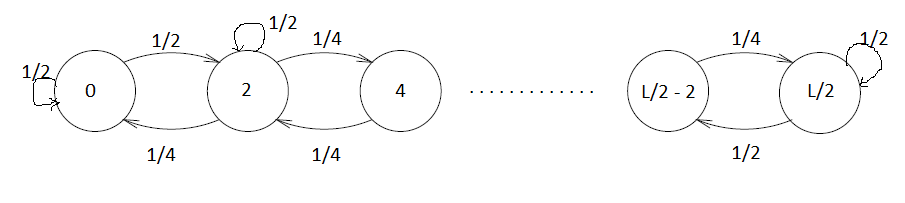
\includegraphics[scale = 0.5]{markovchain.png}
	\caption{Random walk on a finite lattice can be seen as random walk on a circle}
	\label{mc}
\end{figure}
\begin{equation}
D_{L/2}(n+1)=
\begin{cases}
\frac{L}{2} & w.p. \hspace{0.2cm} \frac{1}{2}\\
\frac{L}{2}-1 & w.p. \hspace{0.2cm} \frac{1}{2}
\end{cases}
\end{equation}
\par This Markov chain has a finite number of states from 0 to $\frac{L}{2}$ and hence is positive recurrent. We wish to find the expected time to hit state '0' from the state $\frac{L}{2}$ that is $\mathbb{E}[T_{L/2,0}]$. Since this is the time for two nodes located diammetrically opposite on the circle to meet each other, it will give us an upper bound on the expected time for multiple nodes to meet one another as explained before.
\par Writing the one step transition probabilities, we obtain 
\begin{align*}
	\mathbb{E}T_{20}&=1+\frac{\mathbb{E}T_{20}}{2}+\frac{\mathbb{E}T_{40}}{4}\\
	\mathbb{E}T_{40}&=1+\frac{\mathbb{E}T_{40}}{2}+\frac{\mathbb{E}T_{20}}{4}+\frac{\mathbb{E}T_{60}}{4}\\
	\vdots & \hspace{1cm}\vdots  \hspace{1cm}\vdots \hspace{1cm}\vdots\\
	\mathbb{E}T_{L/2-2,0}&=1+\frac{\mathbb{E}T_{L/2-2,0}}{2}+\frac{\mathbb{E}T_{L/2,0}}{4}+\frac{\mathbb{E}T_{L/2-4,0}}{4}\\
	\mathbb{E}T_{L/2,0}&=1+\frac{\mathbb{E}T_{L/2,0}}{2}+\frac{\mathbb{E}T_{L/2-2,0}}{2}.
\end{align*}
Expressing these set of equations in matrix form, we get,
\begin{equation}
\begin{pmatrix}
\frac{1}{2} & \frac{-1}{4} & 0 & \cdots & 0 & 0\\
\frac{-1}{4} & \frac{1}{2} & \frac{-1}{4} & \cdots & 0  & 0\\
0 &\frac{-1}{4} & \frac{1}{2} & \cdots & 0 & 0\\
\vdots  & \vdots & \vdots & \ddots & \vdots & \vdots \\
0 & 0 & 0 & \cdots & \frac{-1}{2} & \frac{1}{2} 
\end{pmatrix}
\begin{pmatrix}
\mathbb{E}T_{20}\\
\mathbb{E}T_{40}\\
\mathbb{E}T_{60}\\
\vdots\\
\mathbb{E}T_{L/2,0}
\end{pmatrix}
=
\begin{pmatrix}
1\\
1\\
1\\
\vdots\\
1
\end{pmatrix}.
\end{equation}
Solving these system of equations, we will be able to find $\mathbb{E}T_{L/2,0}$. As an example, we give below the calculated values when the two nodes are moving on a circle with 13 vertices.
\begin{equation*}
\mathbb{E}T_{20}=10 \hspace{.5cm} \mathbb{E}T_{40}=16 \hspace{.5cm} \mathbb{E}T_{60}=18
\end{equation*}
In general, for the asymmetric random walk, the expected time for two nodes on diammetrically opposite ends of a circle to meet is obtained by solving for $\mathbb{E}T_{L/2,0}$ in the following system of equations;
\begin{equation}
\begin{pmatrix}
2pq & -pq & 0 & \cdots & 0 & 0\\
-pq & 2pq & -pq & \cdots & 0  & 0\\
0 &-pq & 2pq & \cdots & 0 & 0\\
\vdots  & \vdots & \vdots & \ddots & \vdots & \vdots \\
0 & 0 & 0 & \cdots & 2pq & 2pq 
\end{pmatrix}
\begin{pmatrix}
\mathbb{E}T_{20}\\
\mathbb{E}T_{40}\\
\mathbb{E}T_{60}\\
\vdots\\
\mathbb{E}T_{L/2,0}
\end{pmatrix}
=
\begin{pmatrix}
1\\
1\\
1\\
\vdots\\
1
\end{pmatrix}.
\end{equation}

\section{Simulations}\label{sim}
The two main parameters that determine the broadcast time in a multi node setup are number of nodes and torus length.

\begin{figure}[!ht]
	\begin{center}
		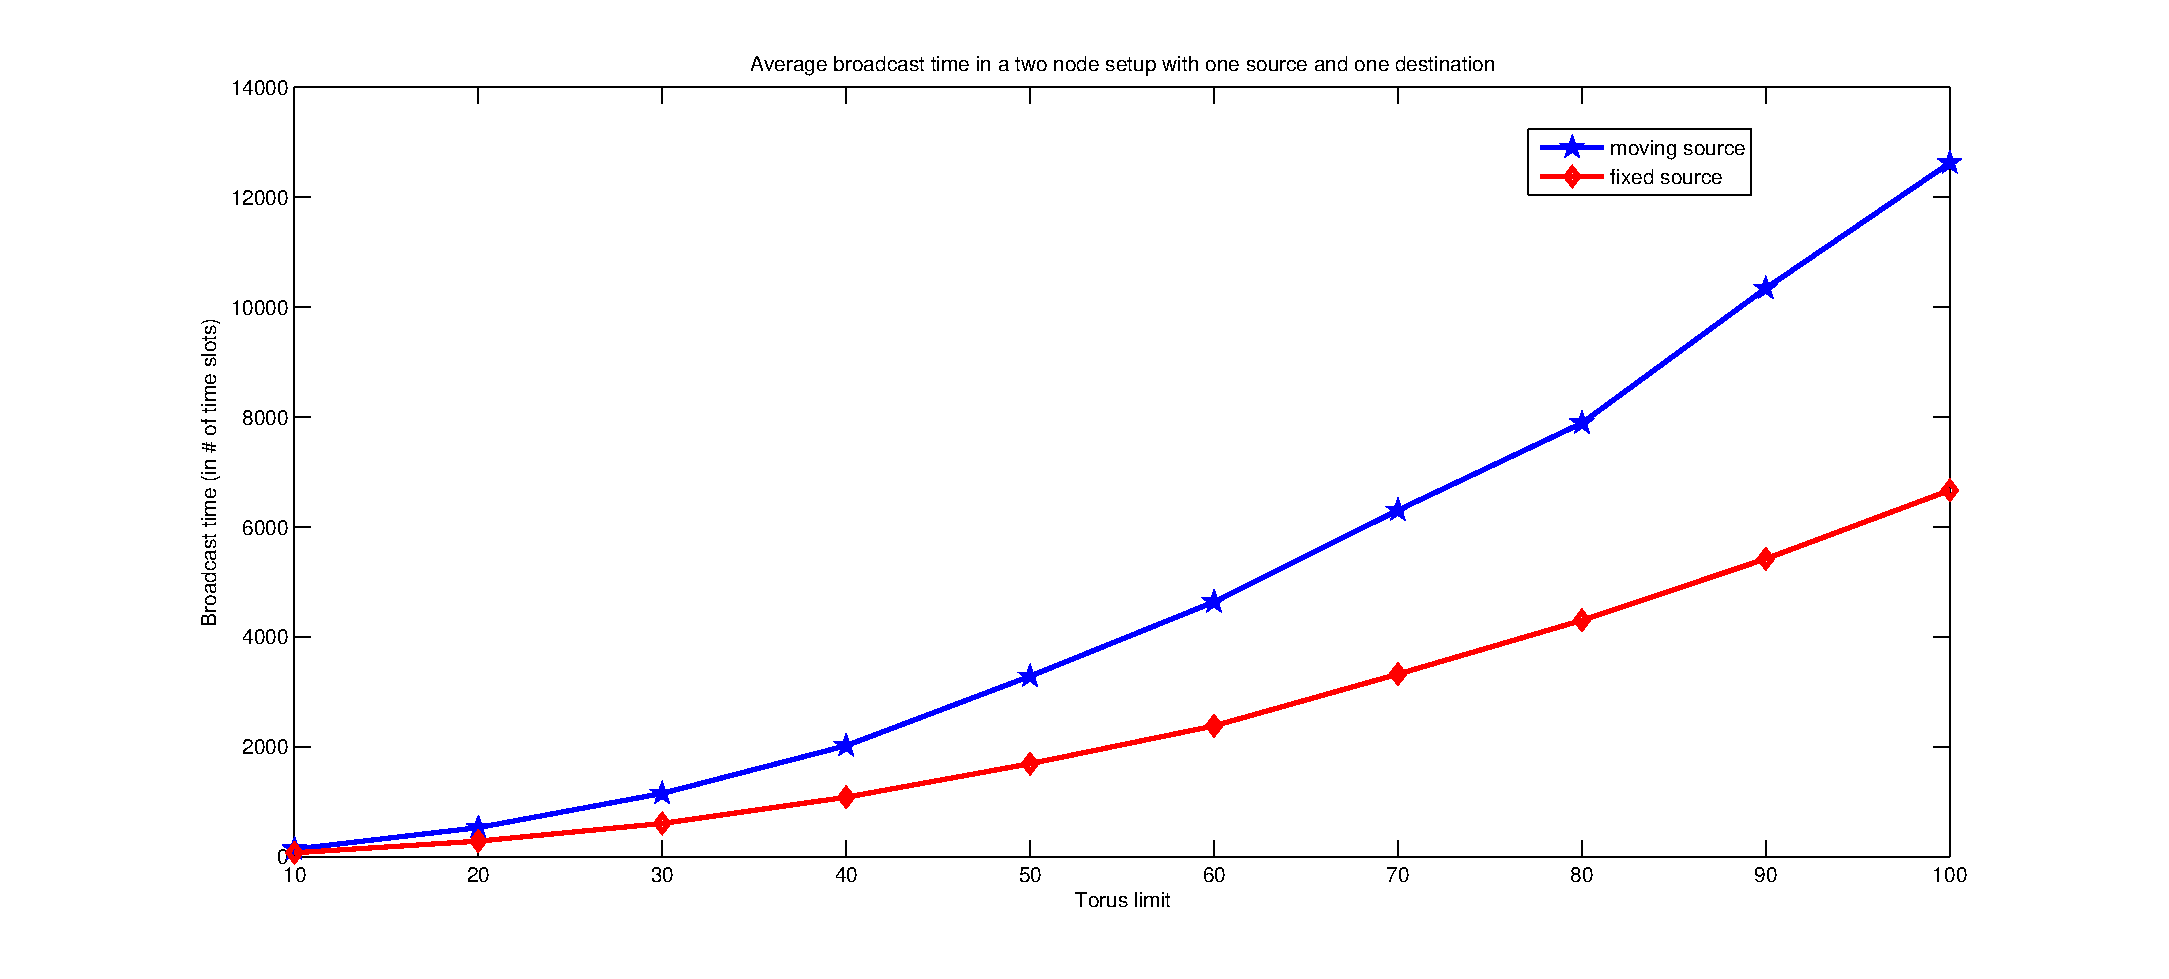
\includegraphics[scale = 0.40]{fixed_move_2nodes.eps}
		\caption{Average broadcast time obtained for 2 node setup, the moving nodes following symmetric random walk. The plots are obtained after 10,000 runs.}
		\label{2node}
	\end{center}
\end{figure}
In Figure \ref{2node}, the limit of the torus length has been varied for a two node setup. Broadcast time for a fixed source is compared with that of the moving source. For a moving source scenario, broadcast time is higher compared to that of stationary source no matter, for a given torus length. The difference between broadcast times for the two scenarios at a given torus length varies as a function of $\sqrt{L/2}$.

\begin{figure}[!ht]
\centering
		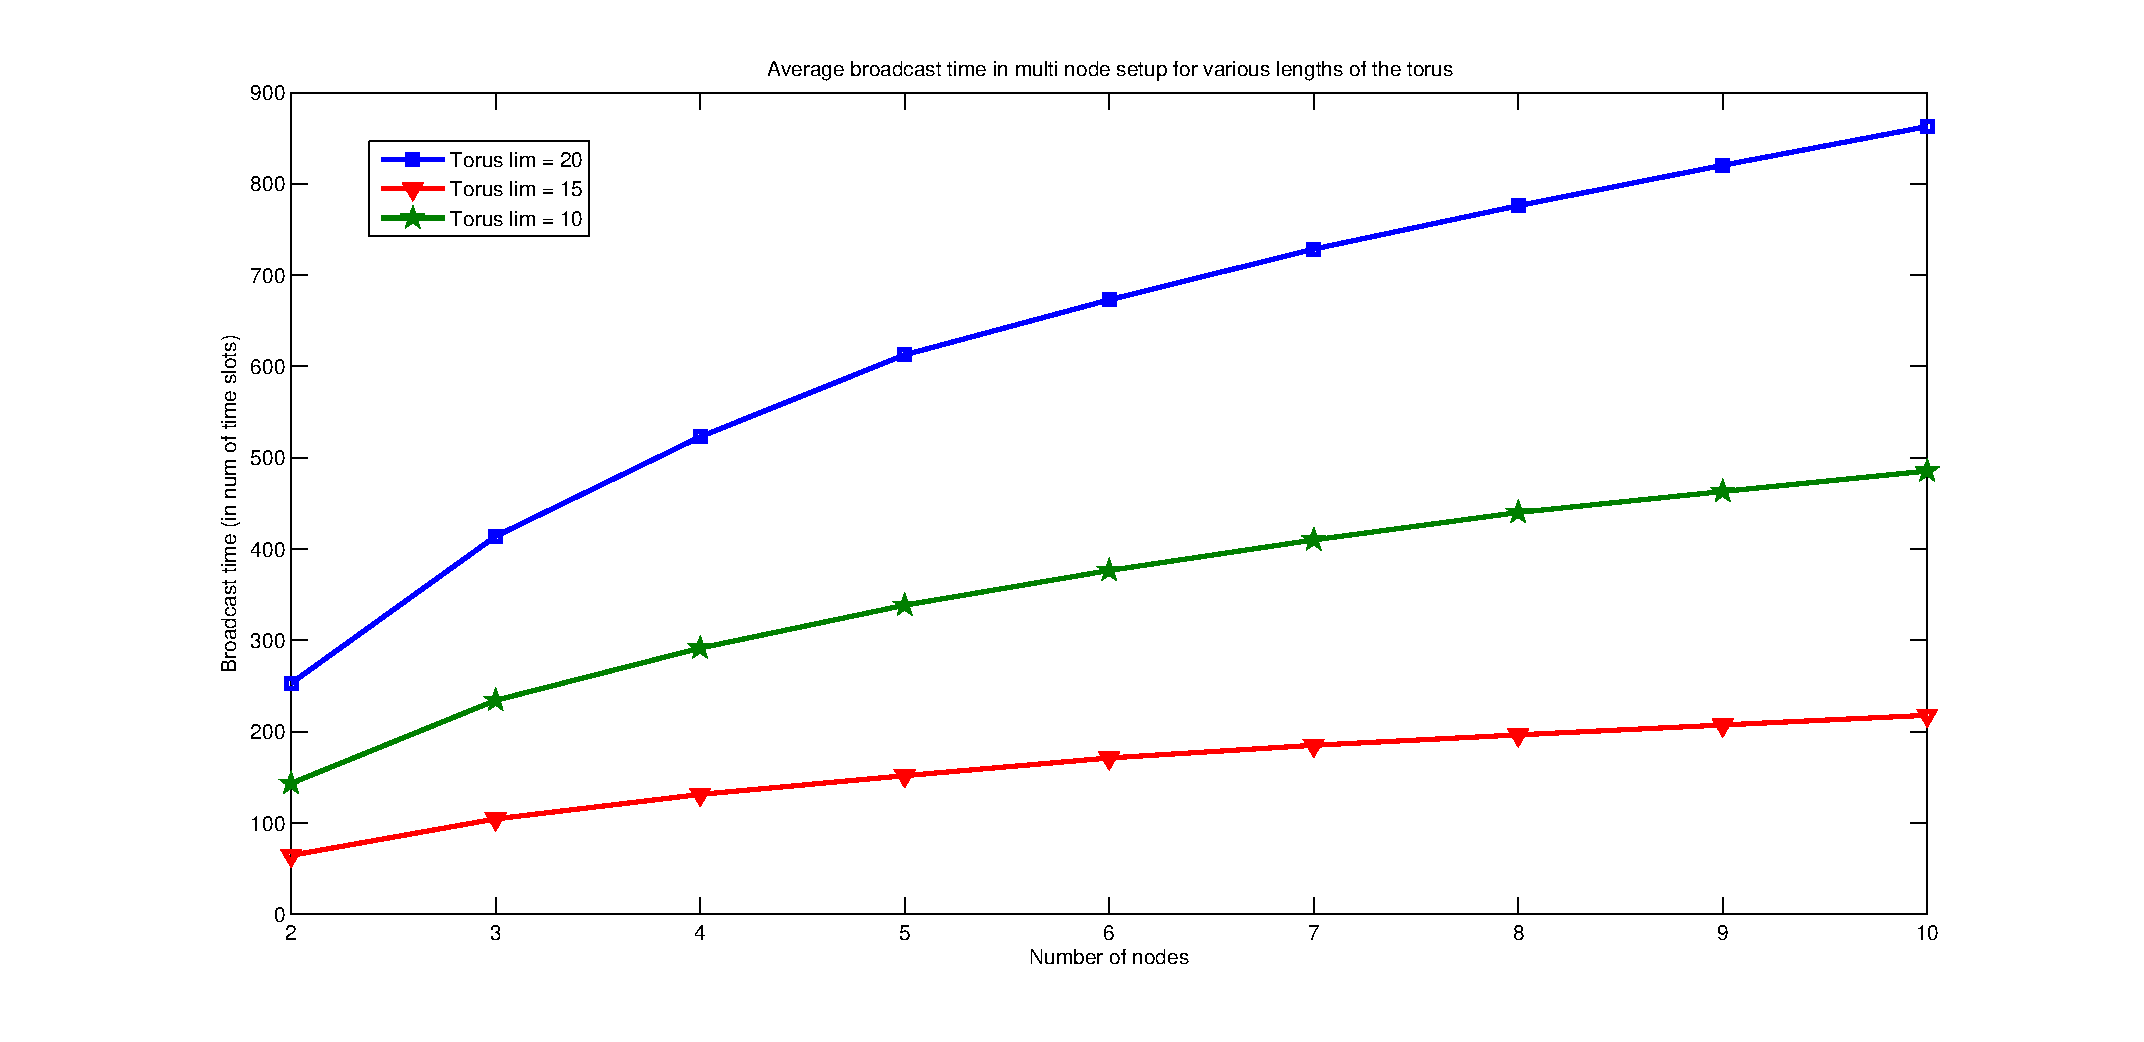
\includegraphics[scale = 0.5]{multi_node_torus.eps}
		\caption{Average broadcast time obtained for multi node setup where the moving nodes follow symmetric random walk. The plots are obtained after 10,000 runs}
		\label{multinode_torus}
\end{figure}

In Figure \ref{multinode_torus}, the number of nodes have been varied to find out the broadcast time for a given length of the torus. As the torus length is increased, the broadcast time increases because the nodes now have more locations to be at. Also, it has been observed that the relationship between broadcast time and the number of nodes is less linear for smaller torus length compared to that of higher torus lengths.

\begin{figure}[!h]
	\begin{center}
		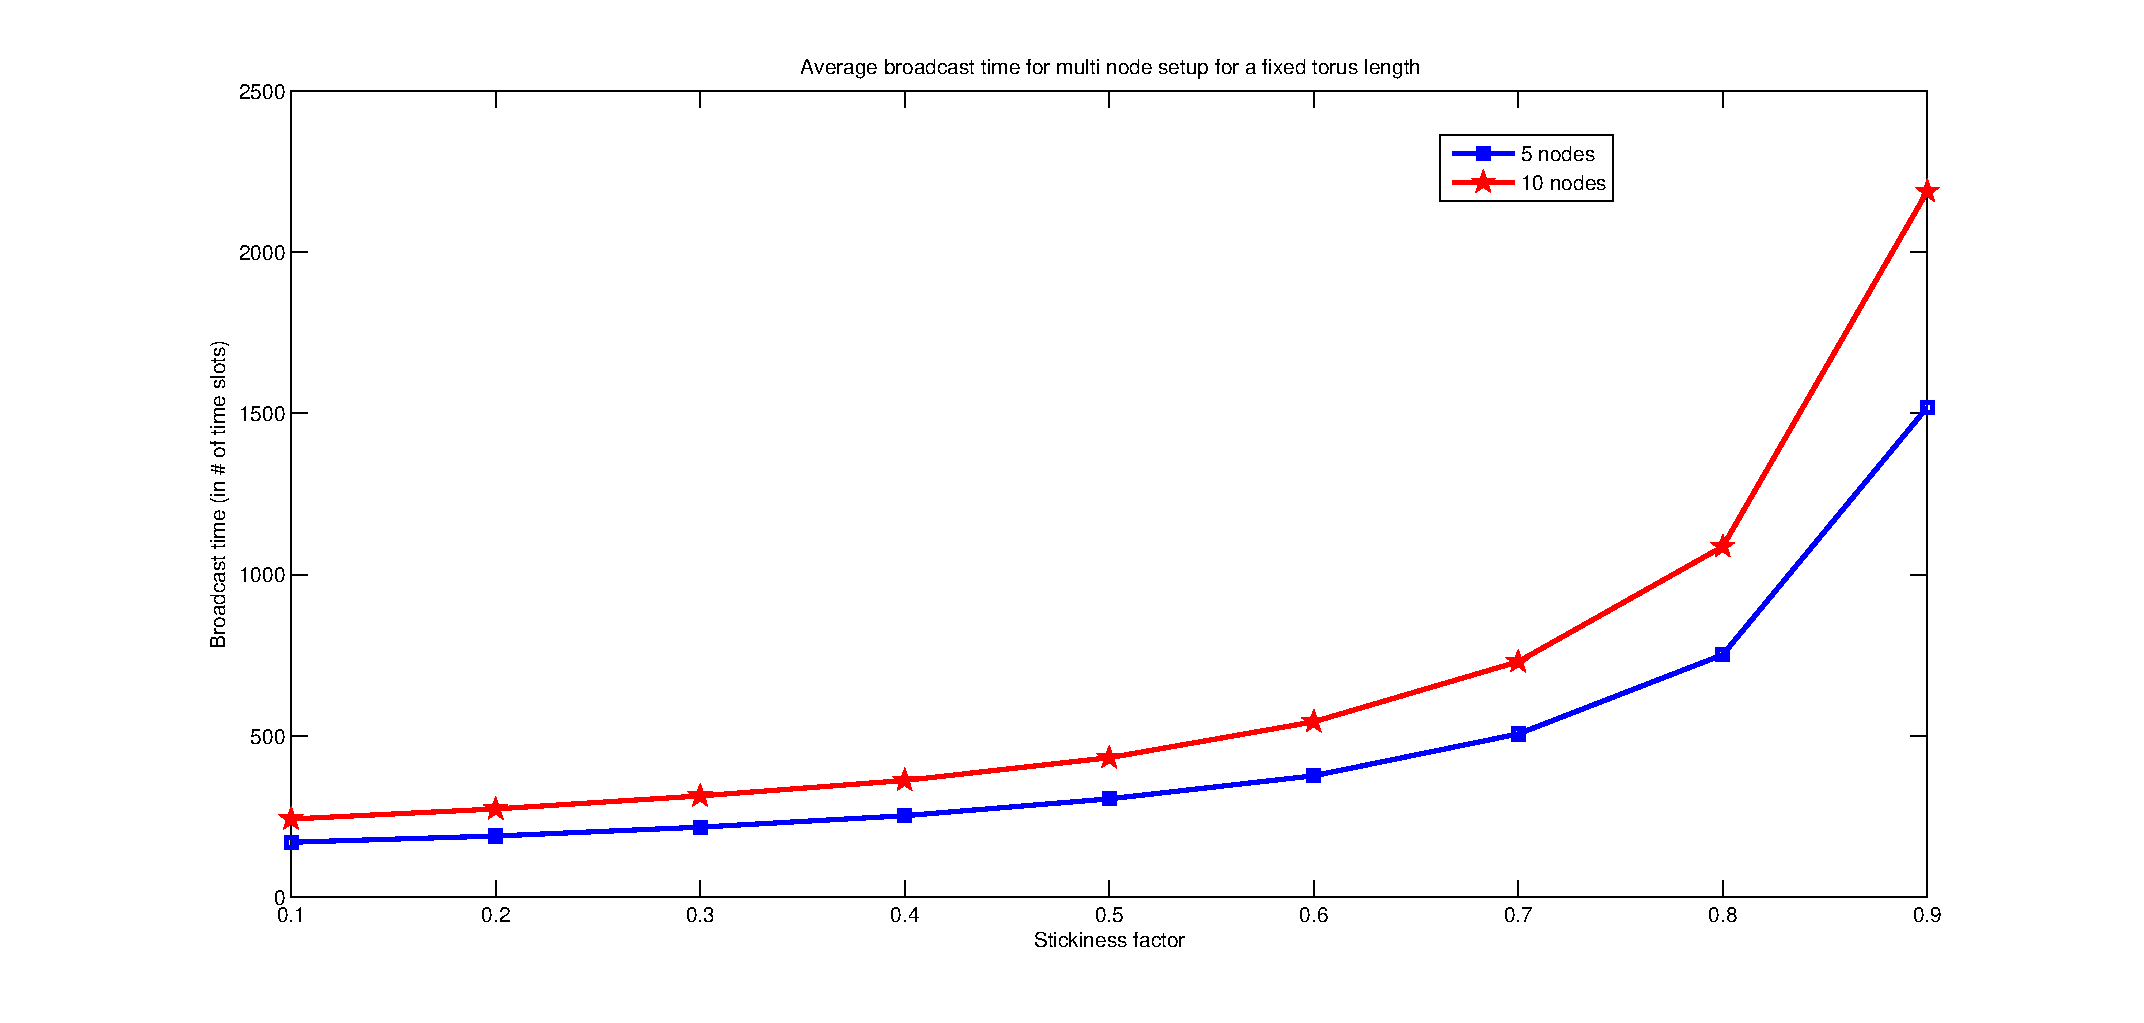
\includegraphics[scale = 0.5]{sticky_comp.eps}
		\caption{Average broadcast time obtained for multi node setup obtained as a function of laziness/stickiness. The plots are obtained after 10,000 runs for a torus length of 21.}
		\label{stickiness}
	\end{center}
\end{figure}

In Figure \ref{stickiness}, broadcast time is plotted as a function of laziness of the nodes. The probability of a node being stationary has been increased for a given number of nodes. It was expected that there will be an optimum amount of stickiness for a given network setup but no such thing has been observed. The broadcast time simply increases with increasing laziness in the network.  
\FloatBarrier


\section{Conclusion}\label{concl}
The following have been accomplished in this project.
\begin{enumerate}
	\item Analysis for two node setup - stationary source, with mobile destination following symmetric and asymmetric random walk.
	\item Analysis for two node setup - mobile source, with mobile destination following symmetric and asymmetric random walk.
	\item Example of calculation of broadcast time for a mobile source and destination for a fixed torus length.
	\item Simulations for two node and multi node setup for all the above.
\end{enumerate}

\section{Future work}\label{fw}
There are several possible extensions of this work.
\begin{itemize}
	\item Extending the analysis for multi node setup. Expected value of broadcast time could be obtained as a function of torus length in this case too.
	\item Analyse and simulate the 2D random walk. The worst initial configuration could then be two groups of clusters, one with information and one without. It would be interesting to find out the expected time for atleast one of the nodes of information cluster to get information from the other cluster.
	\item Observe the advantage or disadvantage the laziness of random walk on the broadcast time in a multi node setup through analysis. 
	\item It would be interesting to analyse and simulate the setup with varying laziness of the nodes.
\end{itemize}
\begin{thebibliography}{5}
	\bibitem{circle2}
	Jeffrey S. Rosenthal, Random Walks on Discrete and Continuous Circles, Journal of Applied Probability 30 (1993), 780–789.
	\bibitem{diaconis}
	Persi Diaconis, Group Representations in Probability and Statistics, Harvard University.
	\bibitem{circle}
	Sven Erick Alm, 'Sim[ple Random walk',April 2002
	\bibitem{ross}
	Sheldon M. Ross, 'Stochastic Processes', Second edition, Wiley Publications.
\end{thebibliography}

\end{document}